\chapter{Efficient verification interfaces and risk-based human escalation}\label{efficient-verification-interfaces-and-risk-based-human-escalation}

On my own site, every agent output arrives as a schema-validated Git diff. The agent cannot write to the production database or publish a page. That architecture places the proposed state transition in an artifact I can read, execute, reject, or revise before it acquires production authority. It provides no evidence that the output is correct. A diff that is easy to approve looks a great deal like a diff that has been checked.

A reviewer skimming that diff is making a cost-benefit decision. Reading every changed branch, reconstructing the intended behavior, running the relevant tests, and checking the result against the task costs far more than a single approval click. When the expected consequence of a missed defect feels remote, that cost difference makes shallow review the rational response, even for a reviewer who intends to be careful.

Vasconcelos et al.~(\href{https://arxiv.org/abs/2212.06823}{2023}) tested this account across five experiments. Their subject was overreliance, the reliance failure in which a person accepts an incorrect AI output. It changed when the economics of checking changed. Participants engaged more when verification required less effort or when the cost of an error became more salient. Explanations reduced overreliance when they altered that calculation. They did not work as a general antidote to misplaced trust.

This result changes the engineering question. Telling reviewers to be more careful treats attention as a personality trait. A review system has to account instead for the price of obtaining evidence, the point at which a person can accept an output, and the finite supply of human judgment. Those are properties of the workflow, and they can be inspected and changed.

Review capacity does not grow because a fleet can produce more patches. Practitioner reports already describe systems generating substantial code volume behind retained human gates. InfoQ reported (\href{https://www.infoq.com/news/2026/03/stripe-autonomous-coding-agents/}{2026}) that Stripe's Minions system produces more than 1,300 production pull requests per week. The figure says nothing about review depth, defect escape, or whether the gate changed any verdict, which is the part I would want to know. It does illustrate the queueing problem. Generation can scale faster than the people authorized to accept its consequences.

I treat this mismatch as three connected design problems. The review surface has to make a correctness claim cheap to challenge. Friction has to interrupt the fast accept loop without taxing every interaction equally. Automated monitors have to concentrate scarce human attention on the cases that warrant judgment, while the verdict stays with a named person. Each intervention changes the cost or the allocation of review. None of them creates correctness.

Nearly all of the empirical oversight results I have used here predate long-horizon agents. In my reading of that work, researchers have rarely tested whether findings about people reviewing suggestions carry over to autonomous actions, although they commonly assume that they do. A code completion that waits for a programmer to accept one function and an agent that edits files, runs commands, revises its plan, and opens a proposed patch create different observability and control problems. The older evidence is useful for identifying mechanisms. It does not settle how those mechanisms behave after autonomy, duration, and action space increase.

The practical standard is therefore narrower than `keep a human in the loop.' A loop can contain a human who sees too little, arrives too late, has no affordable way to check the work, or lacks the authority to stop it. The questions worth asking are concrete. What evidence reaches the reviewer? At which decision is independent judgment required? Which cases consume scarce review time? Who owns the final verdict, and what happens after that person decides?

\section{The price of a check}\label{the-price-of-a-check}

An explanation describes why an output might be right. A verification interface gives the reviewer a practical way to discover that it is wrong. Tests, executable examples, types, continuous-integration gates, sandboxed runs, and evidence placed next to the claim all serve the second purpose. Their value comes from the failures they can expose.

Suppose an agent changes a retry loop. A prose rationale might say that the new backoff prevents overload while preserving responsiveness. A useful review surface shows the changed state machine, the maximum attempt count, the errors classified as retryable, and a test that advances a fake clock through failure and recovery. The reviewer can then challenge specific claims: whether retries stop, whether a non-retryable error escapes immediately, whether cancellation is honored, and whether two workers can duplicate the side effect. The explanation may help locate those claims. The executable evidence does the checking.

The same principle governs evidence presentation. Admission to the review surface and inspection within an artifact are different decisions. A system may correctly decide that logs, traces, generated files, and dependency changes belong in the review packet and still bury the relevant event among thousands of lines. Curating what reviewers see helps only when the omitted material remains reachable and the curation rule itself can be inspected. Otherwise the interface reduces apparent complexity by hiding the evidence needed to falsify the output.

Fok and Weld (\href{https://arxiv.org/abs/2305.07722}{2024}) synthesized the research on explainable AI and reached a compatible but directional conclusion. Explanations rarely produced complementary performance, in which the human and the AI together outperform either one alone, unless the explanation helped the person verify the answer. That literature spans tasks with different error costs, expertise requirements, and verification opportunities, so it does not justify a universal claim that one explanation format will improve code review. It does support a sharper design test. After reading the explanation, what can the reviewer now check that was previously too expensive or unavailable?

Software is unusually favorable under that test. Many software claims admit partial mechanical oracles. A compiler can reject a type error. A property test can generate cases a reviewer would not enumerate. A deterministic replay can expose an ordering fault. A sandbox can show which files and network endpoints an action touched. None of these proves total correctness, but each can move a claim from something the reviewer has to read and trust toward something the reviewer can run and challenge.

The favorable case has strict boundaries. A passing test suite establishes only that the tested behavior passed under the tested conditions. Generated tests can repeat the implementation's mistaken assumption. Type systems encode some properties and omit others. Sandboxes constrain consequences without establishing intent. A green continuous-integration result can itself become a trust signal that accelerates acceptance, even when the changed risk lies outside the suite.

A large diff with weak tests can therefore leave verification more expensive than acceptance. The reviewer has to reconstruct behavior across files, infer unstated requirements, and judge interactions that no executable check covers. Adding a longer reasoning trace increases reading cost without creating an oracle. Under those conditions, the cost-benefit account predicts shallow engagement.

Optimizing first for the completeness of an agent's explanation is therefore the wrong starting move. The useful first step is to identify the claims whose failure matters and ask what artifact could disconfirm each one. For a database migration, that might mean forward and rollback rehearsal against representative data. For an authorization change, it might mean a table of identities and denied actions executed as integration tests. For a concurrent worker, it might mean a trace that records ownership, ordering, retries, and idempotency keys across an injected failure.

The check also needs a sound scope. A changed-file hook that formats or tests only the affected modules can shorten feedback time, but its dependency model has to be correct. When a shared schema changes, the affected set may extend well beyond the edited directory. Cheap verification produced by unsound scoping is an instrumentation artifact. The dashboard becomes greener because the check stopped looking where the failure can occur.

Displayed confidence does not repair that defect. Any confidence signal should be calibrated before it reaches the reviewer, because an uncalibrated percentage adds persuasive precision without dependable information. Calibration remains a prerequisite for presenting the signal, not a substitute for inspecting the claim underneath it. A reviewer still needs to know what event the probability describes, over which population it was estimated, and whether the current case resembles that population.

The cost model includes more than minutes. Verification can require scarce domain knowledge, access to production-like state, coordination with another owner, or the authority to run a destructive rehearsal safely. A one-command check can be computationally cheap and organizationally expensive.

Sarkar et al.~(\href{https://arxiv.org/abs/2208.06213}{2022}) advanced a companion hypothesis that treats verification as the dominant cost of agent-produced software. Their support is anecdotal synthesis and the magnitudes are not quantified, so the hypothesis is useful for inspecting a workflow rather than as a measured law. The more defensible claim is conditional. When generation becomes cheaper while the cost of establishing correctness does not, verification becomes a larger share of the work. Capacity plans that count generated patches but omit review evidence measure supply while ignoring the constrained resource.

The design objective is not that every check becomes effortless, because some claims have no cheap oracle. The objective is to avoid charging reviewers for work the system could have done mechanically, and to make the remaining uncertainty visible. An explanation without a practical check is context. It may orient the reviewer, but it should not be recorded as evidence that the change is safe.

\section{Friction at the decision, not across the workflow}\label{friction-at-the-decision-not-across-the-workflow}

Making a check inexpensive does not ensure that anyone performs it. A reviewer can still form a global rule, something on the order of `this agent is usually right', and apply it to the next output without examining the particulars. The interface then has to interrupt the act of acceptance rather than add ceremony to every step preceding it.

A cognitive forcing function requires deliberate judgment at a point where a person would otherwise rely on a fast heuristic. In an AI review flow, it might require the reviewer to record an independent answer before the system reveals the agent's answer. It might delay the reveal at a consequential checkpoint. It might ask the reviewer to name the expected failure mode before showing test results, or require a specific reason for accepting a risky change. The intervention is worth its cost only when it changes the decision process at the point where overreliance occurs.

Buçinca, Malaya and Gajos (\href{https://arxiv.org/abs/2102.09692}{2021}) tested cognitive forcing functions in a controlled experiment with 199 participants. The interventions reduced overreliance where explanations did not, but they did not eliminate it. The most effective interventions were also rated least favorably. Benefits accrued disproportionately to participants with high Need for Cognition, a measured tendency to engage in effortful thought. Friction changed behavior, but it imposed a real usability cost and did not reach everyone equally.

This unpopularity is not an incidental implementation problem. Effective friction blocks the shortest path through the task. Users therefore experience its mechanism as inconvenience. A team that evaluates the gate only through satisfaction scores will select against the property that makes it work. A team that ignores usability will accumulate workarounds, perfunctory responses, and political pressure to remove the gate.

The comparison worth running has three terms: the defect detection gained at a defined decision, the delay and cognitive load imposed there, and the behavior that appears after repeated use as the amount of friction changes. A forcing function can improve an experimental average while training experienced reviewers to enter meaningless text. It can also move acceptance to a different channel where the decision is less observable. The control has to be evaluated as part of the workflow it changes.

Barke et al.~(\href{https://arxiv.org/abs/2206.15000}{2023}) ran a grounded-theory study of twenty programmers that suggests where to target the intervention. They observed a bimodal pattern in code-generation interactions. In acceleration mode, the programmer believed the plan was already understood and used the model to move faster, and validation tended to be shallow. In exploration mode, the programmer used suggestions to discover an approach and already engaged in more deliberation.

This distinction offers a better allocation rule than a uniform gate. Requiring an independent judgment during acceleration can interrupt a reflexive accept loop. Requiring the same ceremony during exploration may add cost to a mode in which programmers already compared, revised, and rejected suggestions. Uniform friction is administratively simple, but it spends reviewer tolerance without regard to the behavior it is meant to change.

Barke et al.~(2023) studied suggestion-level interaction, not autonomous agents producing multi-file diffs after long trajectories. Acceleration and exploration may coexist within one agent run. A programmer might explore the architecture, delegate an implementation, and then accelerate through review because the overall plan feels familiar. The suggestion-level split is a useful hypothesis for instrumenting such a workflow, but its transfer to autonomous-agent diffs remains untested.

A practical system needs an observable proxy for the decision context without pretending to read the reviewer's mind. High-impact file classes, a previously approved plan, repeated acceptance from the same agent, a large generated diff, or a short interval between presentation and acceptance can each identify a candidate checkpoint. Each proxy can also be wrong. Diff size is not risk, speed is not negligence, and familiarity can reflect genuine expertise.

Targeting should therefore be treated as an experiment with explicit failure measures. Record where the intervention appears, whether the reviewer changes or rejects the output, how long the decision takes, whether later defects concentrate in bypassed cases, and whether users route work around the gate. Segment the results by reviewer experience and task type. Each added segment is another comparison, so the analysis needs the multiplicity correction Chapter 1 describes before a subgroup difference is read as real. An aggregate acceptance-rate change cannot show whether the intervention improved judgment or merely annoyed one group into abandoning the workflow.

Time pressure deserves separate treatment. Rosbach et al.~(\href{https://arxiv.org/abs/2411.00998}{2024}) studied computational pathology and found that time pressure increased the severity of automation-bias errors while leaving their frequency unchanged. That setting does not establish the same effect in software review. It does point to a control mistake. Adding a forcing function while preserving an impossible service deadline can produce fewer opportunities for reflection precisely on the cases whose consequences are largest. Shielding a checkpoint from time pressure can matter as much as adding the checkpoint.

The decision prompt itself should solicit evidence tied to the action it authorizes. ``Have you reviewed this?'' can be answered with a checkbox. ``Which authorization boundary changed, and which denied case demonstrates that it remains closed?'' asks for a claim tied to a check. The answer can still be wrong, but the interface makes shallow assent harder to reconcile with the action it authorizes.

Forcing functions also need escape routes. An emergency response may justify bypassing an independent pre-commit judgment, but the bypass should still identify the owner, the reason, and the follow-up state. A gate with no exception can be unsafe when delay is costly. A gate whose exception leaves no durable record becomes optional whenever pressure rises.

Chapter 16 examines how to determine whether documented gates still affect execution. The narrower conclusion here is that friction is unpopular by construction. Its continued presence and actual use therefore cannot be inferred from the workflow diagram.

\section{Escalation as measured triage}\label{escalation-as-measured-triage}

Kale et al.~(\href{https://arxiv.org/abs/2508.19461}{2025}) reported that targeted escalation improved the true-positive rate over blanket oversight at a 0.01 false-positive rate, a gain the paper records as approximately 15 percent. Blanket oversight does not bound the true-positive rate from above at fixed human capacity. Attention spread across every case reduces per-case scrutiny and raises misses, while targeting spends the same attention on fewer cases. Their hybrid hierarchical and sequential scaffolds also allowed weaker models to monitor stronger agents.

That result is unusually relevant, because it evaluated the allocation of oversight rather than only asking whether a judge can classify isolated outputs. Its setting was a covert-misbehavior arena. It was not production code review, and the reported operating point should not be treated as a deployment guarantee. The improvement is also one comparison at one operating point, and a monitor that gains at a 0.01 false-positive rate need not gain by the same margin at another threshold.

The basic allocation problem exists outside that arena. When every agent action receives the same human review depth, the number of actions determines the review burden. A fleet can then increase output until reviewers skim, queues stall, or teams weaken the gate. Blanket oversight preserves the appearance of equal scrutiny while degrading the scrutiny available per case.

Targeted escalation changes the unit of human work. Automated monitors inspect the full stream, and humans receive the cases the monitors flag. An escalation route runs from a flag to a named decision owner, a verdict, and a defined resumption state. Without those elements, a flag is a notification. It can remain unread, bounce among teams, or leave execution suspended indefinitely.

A monitor scaffold assigns each kind of detection to the least complex mechanism capable of checking it. Deterministic rules handle exact violations. A model judge applies a fixed rubric to contextual cases. An agent judge examines live traces when the decision depends on sequence, changing state, or tool interaction. Human reviewers calibrate the layers and own the final verdict. Kale et al.~(2025) measured the value of scaffolding itself. The ordering of these three layers is a design convention drawn from one practitioner account, with no independent measurement behind it.

A deterministic rule can establish that an agent wrote outside an allowed directory, attempted a forbidden operation, or omitted a required approval token. Asking a model to infer an exact violation adds variance without adding useful judgment. A model judge becomes appropriate when the rubric requires contextual interpretation, such as whether a migration plan includes a credible rollback for the affected data path. An agent judge is reserved for cases in which no single artifact contains the evidence, such as whether a sequence of individually allowed actions collectively bypassed a control.

Each layer has to expose its evidence to the next. A rule should report the event and the policy clause it matched. A model judge should return the rubric criterion, the supporting trace span, and the uncertainty relevant to escalation. An agent judge should preserve the observations and intermediate actions needed to reconstruct its conclusion. A bare risk score forces the human to repeat the discovery work or to accept the classifier's authority without a check.

\begin{verbatim}
kind of detection
    -> least complex mechanism capable of checking it
        |
        +-> exact violations
        |   -> deterministic rules
        |      -> event + matched policy clause
        |
        +-> contextual cases
        |   -> model judge with fixed rubric
        |      -> criterion + trace span + uncertainty
        |
        +-> sequence + changing state + tool interaction
            -> agent judge examines live traces
               -> observations + intermediate actions

human reviewers -> calibrate the layers -> final verdict
bare risk score -> human repeats the discovery work
\end{verbatim}

Calibration follows the Chapter 5 procedure. Select the operating point against an expert-labeled stratified matched control set that represents the consequential case types, including rare failures. Report the true-positive rate at the chosen false-positive rate and retain the confusion matrix by stratum. Both rates are estimates from a finite labeled sample, and a stratum with few labeled cases yields a wide uncertainty interval. Re-run the evaluation when the agent, rubric, tools, environment, or case mix changes. An overall accuracy number is especially misleading when most actions are benign and the human queue is constrained by false positives.

The queue budget is part of the operating point. At a 0.01 false-positive rate, a monitor applied to one hundred actions creates a different human burden from the same monitor applied to one million actions. Base rates and action volume determine the absolute number of false alarms. When the flagged condition is rare, that number is drawn from a much larger population of benign actions. False alarms can therefore outnumber correct flags even at a low false-positive rate, which is the prevalence effect Chapter 5 describes for graders. A statistically respectable rate can still exhaust the review team.

\begin{figure}
\centering
\pandocbounded{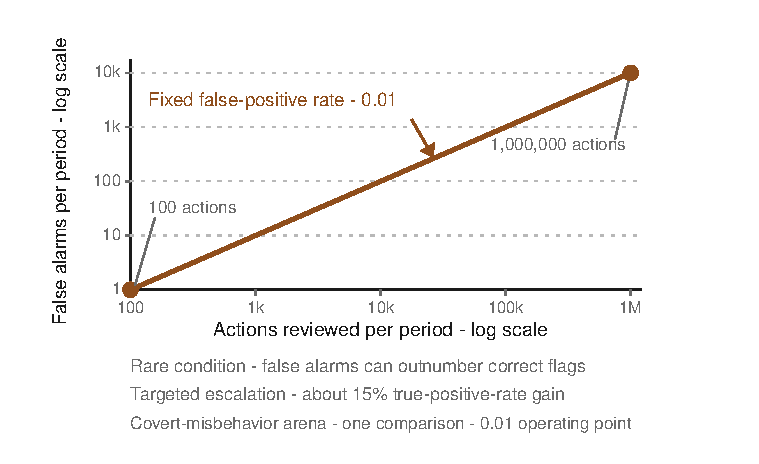
\includegraphics[keepaspectratio,alt={At fixed 0.01 false-positive rate, false alarms rise from 1 among 100 actions to 10,000 among 1,000,000 and can outnumber correct rare-event flags; targeted escalation adds about 15\% true-positive rate in one covert-misbehavior arena.}]{figures/ch15-queue-budget.pdf}}
\caption{At fixed 0.01 false-positive rate, false alarms rise from 1 among 100 actions to 10,000 among 1,000,000 and can outnumber correct rare-event flags; targeted escalation adds about 15\% true-positive rate in one covert-misbehavior arena.}
\end{figure}

False alarms scale with action volume and base rates. The approximately 15\% escalation gain comes from one covert-misbehavior-arena comparison at a 0.01 operating point.

Escalation is therefore a budgeted online decision. The system has to choose, as cases arrive, which uncertainty deserves scarce human attention now. That choice can account for expected consequence, novelty, reversibility, monitor disagreement, and the availability of a qualified owner. These inputs do not justify an opaque semantic risk formula. They define the evidence given to the judge and the explicit policy constraints applied to the queue.

My own orchestration fleet uses a related division of labor. Mechanical work proceeds autonomously, and judgments the system should not make unilaterally are collected in a structured morning decision ledger. The system does not silently resolve those entries. The design reserves interruptions for entries that need a person. I have not measured maintainer minutes, scrutiny depth, or escaped-defect rate, so the attention saving remains a design claim rather than a demonstrated outcome.

The associated wake-up contract makes the route more specific. The fleet should wake me for suspected wrong calls and for decisions about scope or trust. It should not wake me for passing runs or routine plumbing. A request has to state the outcome at stake, present a decision answerable in one line, list the options and the recommendation, and explain why the system cannot resolve the matter itself. The success criterion is behavioral. Engineers should not learn to filter the messages out.

This contract separates notification quality from verdict authority. A monitor may decide that a case meets the escalation rule. It should not quietly convert that classification into the substantive decision under review. The person named on the route must be able to reject the work, request evidence, narrow the scope, or authorize resumption. Naming an owner who cannot do these things assigns accountability without control.

The resumption state deserves explicit design, because asynchronous review creates races. If an agent continues acting while its escalation is pending, a later rejection may arrive after dependent actions have executed. If execution stops globally, an unrelated low-risk queue can be blocked by one ambiguous case. The route should state whether the affected action, trajectory, repository, or fleet pauses, which state is durable, and which decision token releases it.

Observed failure paths should determine checkpoint placement. When damaging actions become irreversible at deployment, a checkpoint after deployment can only document what happened. When the common failure begins as a plan silently expands its scope, waiting until the final diff makes reconstruction expensive. The companion pattern is narrow. Place human checkpoints where failure evidence shows that intervention can still change the outcome.

Human skill is another boundary. A reviewer who handles only rare anomalies may lose familiarity with ordinary system behavior, while automation inherits the routine cases that once maintained that familiarity. Bainbridge (\href{https://doi.org/10.1016/0005-1098(83)90046-8}{1983}) described this problem for industrial process control in ``Ironies of Automation.'' Its transfer to software-agent oversight is an analogy rather than a measured result on software work. It nevertheless identifies a design question that triage cannot answer alone. How will the person expected to intervene retain the knowledge needed to recognize and correct an abnormal state?

Xie et al.~(\href{https://arxiv.org/abs/2408.01703}{2024}) advanced a thinly supported companion proposal. Agent actions can be rendered as live state so that a reviewer inspects a trajectory before it terminates. The support is one prototype-scale item and does not establish improved oversight. The proposal is useful as a design prompt when late reconstruction has repeatedly failed, provided that the live view preserves the durable trace rather than replacing it.

Monitoring can alter the behavior it measures. An agent that knows it is being watched may adapt to the evaluation frame. I treat that possibility as a design caution and not as a measured result from Kale et al.~(2025), whose reported result was that monitor scaffolding mattered more than monitor awareness. In my own evaluation harnesses, I therefore use de-framed prompts that omit evaluation vocabulary, so the acting agent receives no cue to behave differently because it is being assessed. Removing that cue is a design precaution against one measurement effect, but it provides no proof that the resulting behavior matches unobserved production behavior.

Judge drift creates a second measurement problem. Deterministic rules drift when policy or event schemas change. Model judges drift when the evaluated distribution, the model version, or the rubric interpretation changes. Agent judges can drift most severely, because their behavior depends on a longer sequence of observations and actions. A monitor calibrated last quarter may preserve its interface while changing which cases reach humans.

Layering redistributes detection work, but it does not resolve who judges the judges. Human owners need sampled review of unflagged cases to estimate misses, adjudication of flagged cases to measure false alarms, and versioned records connecting each verdict to the monitor configuration that produced it. The sample cannot consist only of easy negatives. It has to include strata in which the monitor is likely to fail and cases drawn after relevant system changes. The sampling unit is the action or trajectory the monitor scored, and estimates from a stratified sample have to be weighted back to the deployed case mix before they describe the monitor in production.

These audits do not require blanket human oversight of every action. They require enough independent labels to estimate whether the chosen operating point still holds. When the estimate degrades, the response may be recalibration, a narrower deployment boundary, a new deterministic check, a rubric revision, or more human review. The correct response depends on the failure mechanism, and `use a stronger judge' is not a diagnosis.

\section{An operating protocol}\label{an-operating-protocol}

Start with one consequential agent workflow. Identify the acceptance decision that transfers authority from proposed work to an effect: merge, deploy, publish, modify data, contact a customer, or change another system's state. Name the person or role that owns that decision. When no one can be named, escalation cannot end in an accountable verdict.

For that workflow, list the claims a reviewer must establish before acceptance. Attach a falsification artifact to each claim where one is available: a test, a typed interface, a replay, a trace, a sandbox result, a policy match, or an executable example. Mark the claims that still depend on expert judgment. Do not count an explanation as evidence unless it makes one of those checks possible.

Measure the review path before adding friction. Record how long evidence takes to obtain, which tools or permissions it requires, where reviewers abandon the check, and which failures remain invisible after a green run. The objective is to find the cases in which the system charges a person for mechanical work or presents confidence without a reachable basis. No universal review-time target applies.

Place a forcing function at the accept decision for the cases in which shallow validation is plausible and consequential. Require an independent judgment or a claim-specific response before revealing the agent's recommendation. Preserve an explicit emergency bypass with an owner, a reason, an affected scope, and a follow-up state. Evaluate detection, delay, bypass, and workarounds together. Satisfaction alone will select for the gates that interfere least.

Build the monitor scaffold from exact checks outward. Use deterministic rules for exact policy violations, a model judge with a versioned rubric for contextual classification, and an agent judge only when sequential interpretation is necessary. Make every layer return the evidence a human needs to challenge it. Calibrate the stack against an expert-labeled stratified matched control set, choose and record the operating point, and translate the rates into expected queue volume at the actual base rate.

Define the escalation route as part of deployment. A flag should identify the decision owner, the outcome at stake, the evidence, the available options, the recommended action, the reason automation cannot decide, the state that is paused, and the event that resumes execution. Test the route by processing a real rejection through it. When the owner cannot stop or revise the action, assign authority before assigning accountability.

Sample both flagged and unflagged cases after deployment. Compare human verdicts with monitor decisions by risk stratum and monitor version. Recalibrate after material changes to agents, tools, rubrics, or workload, and examine whether awareness of monitoring changes behavior. Budget practice for the humans who must handle rare failures. A name in an escalation table does not preserve operational skill.

\section{Sources and evidence}\label{sources-and-evidence}

The evidence class and strength on each entry below come from its catalog record. Author-system cases in this chapter are narrative illustration and are not part of the evidence base.

\subsection{Building verification surfaces so verifying costs less than blind acceptance}\label{building-verification-surfaces-so-verifying-costs-less-than-blind-acceptance}

\begin{itemize}
\tightlist
\item
  lit/strong: Vasconcelos, H., Jörke, M., Grunde-McLaughlin, M., Gerstenberg, T., Bernstein, M., Krishna, R. (2022/2023). Explanations Can Reduce Overreliance on AI Systems During Decision-Making. PACM HCI 7(CSCW1). arXiv:2212.06823. Five experiments treat overreliance as a cost-benefit choice and find greater engagement when verification is cheaper or stakes are higher.
\item
  lit/directional: Fok, R., Weld, D.S. (2023/2024). In Search of Verifiability: Explanations Rarely Enable Complementary Performance in AI-Advised Decision Making. AI Magazine 45(3). arXiv:2305.07722. Across the XAI-reliance literature, explanations help only insofar as they enable verification.
\item
  Corroboration: the author's website, ``Two retrieval systems write this site'' (2026-06-10), an author-owned anecdotal account of schema-validated agent output landing as a git diff that serves as the review gate, and an unpublished internal record of the author's agent-workflow system. Both are narrative only and neither is an admitting basis. Dossier items corroborate only.
\end{itemize}

\subsection{Putting the forcing function at the accept decision, aimed at acceleration mode}\label{putting-the-forcing-function-at-the-accept-decision-aimed-at-acceleration-mode}

\begin{itemize}
\tightlist
\item
  lit/strong: Buçinca, Z., Malaya, M.B., Gajos, K.Z. (2021). To Trust or to Think: Cognitive Forcing Functions Can Reduce Overreliance on AI in AI-assisted Decision-making. PACM HCI 5(CSCW1), 188. arXiv:2102.09692. Cognitive forcing functions reduced overreliance where explanations failed (N=199).
\item
  lit/directional: Barke, S., James, M.B., Polikarpova, N. (2022/2023). Grounded Copilot: How Programmers Interact with Code-Generating Models. PACMPL 7(OOPSLA1). arXiv:2206.15000. Grounded theory from 20 programmers supports the suggestion-level acceleration/exploration split. Transfer to autonomous-agent diffs is untested. This directional item is the only source for the chapter's targeting rule.
\item
  Corroboration: none on record.
\end{itemize}

\subsection{Escalating only monitor-flagged cases to a human who owns the verdict, with a scaffolded monitor}\label{escalating-only-monitor-flagged-cases-to-a-human-who-owns-the-verdict-with-a-scaffolded-monitor}

\begin{itemize}
\tightlist
\item
  lit/strong: Kale, N., et al.~(2025). Reliable Weak-to-Strong Monitoring of LLM Agents. arXiv:2508.19461. Targeted escalation adds approximately 15\% TPR at FPR=0.01. Hybrid hierarchical-sequential scaffolds let weaker models monitor stronger agents. The paper reports that scaffolding mattered more than monitor awareness; the awareness caution in this chapter is my design caution, not a result from this paper. The setting is a covert-misbehavior arena, not production code review. This is the sole admitted evidence item for the whole grouping.
\item
  Corroboration: the author's website, ``Running my own agent city on Slack'' (2026-06-16), an author-owned anecdotal account of mechanical work proceeding autonomously while judgment calls accumulate in a decision ledger for a human; the author's website, ``WF2026: evals are the new CI'' field notes, an account distilled from other people's conference talks of a three-layer judge stack with a human owning the verdict; and unpublished internal context notes. None is an admitting basis. The conference-talk-derived account was demoted out of the evidence base and is not citable as independent support. The chapter's three-layer scaffold ordering rests on it and on nothing stronger. Dossier items corroborate only.
\end{itemize}

\subsection{Companion material carried in-text but not taught as a pattern}\label{companion-material-carried-in-text-but-not-taught-as-a-pattern}

\begin{itemize}
\tightlist
\item
  lit/strong: Rosbach, E., Ganz, J., Ammeling, J., Riener, A., Aubreville, M. (2024). Automation Bias in AI-Assisted Medical Decision-Making under Time Pressure in Computational Pathology. arXiv:2411.00998. This is the basis for the time-pressure paragraph. The setting is computational pathology, not software review.
\item
  lit/directional: Bainbridge, L. (1983). Ironies of Automation. Automatica 19(6), 775-779. \url{doi:10.1016/0005-1098(83)90046-8}. This is the single source behind the skill-retention paragraph. The evidence is pre-AI and industrial. Transfer to code review is analogical.
\item
  lit/anecdotal: Sarkar, A., et al.~(2022). What is it like to program with artificial intelligence? PPIG 2022. arXiv:2208.06213. This is the basis for the companion hypothesis that verification is the dominant cost. The magnitudes are not quantified.
\item
  lit/directional: Xie, L., Zheng, C., Xia, H., Qu, H., Zhu-Tian, C. (2024). WaitGPT: Monitoring and Steering Conversational LLM Agent in Data Analysis with On-the-Fly Code Visualization. UIST 2024. arXiv:2408.01703. This prototype-scale single item is the basis for the live-state proposal and the thinnest support in the chapter. Transfer to arbitrary code agents requires an operation-level abstraction that may not exist.
\item
  explorer/directional: DeepRare (Zhao 2026); Manager Agent (Masters 2025, arXiv:2510.02557); NIST AI RMF.
\item
  explorer/directional: Bounded Autonomy for Enterprise AI (Sohail 2026, arXiv:2604.14723).
\item
  explorer/directional: AMBIPOM human-LLM co-planning (He 2026, arXiv:2605.23023).
\item
  explorer/directional: Token Budgets (Khan 2026, arXiv:2606.04056). Together, the four explorer items support only the direction of the checkpoint-placement claim. None is strong.
\item
  Corroboration: an unpublished internal record of the author's repository-scale benchmark, an unpublished internal record of the author's background-agent review pipeline, and unpublished internal context notes corroborate the checkpoint-placement claim as narrative only. Dossier items corroborate only.
\end{itemize}

\subsection{Opening scene}\label{opening-scene}

\begin{itemize}
\tightlist
\item
  practitioner/corpus-verified: InfoQ, ``Stripe Engineers Deploy Minions, Autonomous Agents Producing Thousands of Pull Requests Weekly,'' 2026-03-20, \url{https://www.infoq.com/news/2026/03/stripe-autonomous-coding-agents/}. Reports over 1,300 production pull requests per week with human review retained. Carried as scale context; it reports no measure of review depth or defect escape.
\end{itemize}
